\chapter{Generic Dataflow Analysis Framework}

This chapter summarizes the basic considerations behind the ROSE dataflow framework as well as how its API can be used to implement inter- and intra-procedural dataflow analyses. It is oriented towards potential users of the framework.

\section{Basics of DataFlowAnalysis}
\label{basics_dfa}
Dataflow analysis is a technique for determining an application’s possible states at various points in a program. It works as a fixed-point iteration over a space of possible facts about each node in the application’s Control Flow Graph (CFG). The algorithm starts with no information about each node and iterates by accumulating all the constraints on the application's state at each node until it reaches a fixed point where no additional constraints can be discovered. The designer of a given dataflow analysis must specify an abstract representation of the set of all possible application states that maintains the relevant details of the state (e.g. whether a variable has a constant value or the linear relationships between variable pairs), while igoring the rest. For example, a state abstraction for the constant propagation analysis may have three different values: the special symbol $\bot$ if the variable is uninitialized, a numeric value if this is the only value the variable may hold at a given CFG node or $\top$ if it may have more than one value. More sophisticated abstractions represent application state using polyhedral constraints or predicate logic.  Further, the designer must specify a ``transfer'' function that maps the abstract state before any application operation to the state after it. For example, if before statement $i++$ it is known that $i==n$ then after the statement it is known that $i-1==n$.  To deal with control flow the designer also specifies a meet function that conjoins the abstract states along multiple control paths. For example, if at the end of the {\scriptsize if} branch of a conditional it is known that i=5 and at the end of the {\scriptsize else} branch i\textless10, the strongest fact that is true immediately after both branches of the conditional is 5 $\le$ i \textless 10.
~\\
The set of possible abstract states must form a lattice, which is a partial order where for any pair of elements there exists a unique least upper bound. Intuitively, states that are lower in the partial order represent fewer constraints on the application state and higher states represent more constraints. The special state $\bot$ corresponds to the least state in the partial order, where the application has done nothing to constrain its state (e.g. all variables are uninitialized). 
The meet function must guarantee the uniqueness of the least upper bound and the transfer function must be monotonic (if A$\le$B then transfer(A)$\le$transfer(B)). The dataflow fixed-point iteration ensures that the abstract state of every CFG node rises monotonically as it incorporates information about more possible application behaviors. When the analysis reaches a fixed point, the abstract state at each CFG node corresponds to the tightest set of constraints that are can be specified by the abstraction about the application state at that location.

\begin{figure}
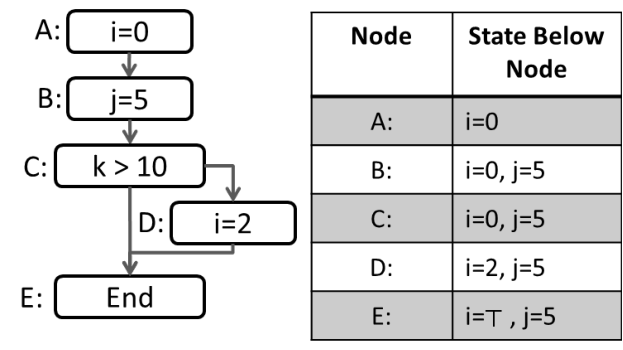
\includegraphics[scale=0.7]{\TutorialExampleDirectory/dfa_cpa}
\caption{Example of a constant propagation analysis.}
\label{Tutorial:dfa_cpa}
\end{figure}

For an intuition about how dataflow analyses work, ~\ref{Tutorial:dfa_cpa} presents an example of a constant propagation analysis. The CFG is on the left and the table on the right shows the fixed-point solution of the abstract state immediately after each node. At each node the abstract application state records for each variable one of the following values: (i) $\bot$, which indicates that the variable is uninitialized, (ii) a specific constant value if the variable may only have this value at node n or (iii) $\top$ which indicates that the variable may have more than one value (i.e., is not representable as a single constant).It shows that immediately after node A it is known that i=0 and similarly after node B, i=0 and j=5. The same is true after node C since it has no side-effects and after the assignment in node D, the state changes to i=2, j=5.  When the two conditional branches meet, the abstract state is the union of the states on both branches: the strongest assertions that are true of both states. Since j has the same value and i has two different values, the abstract state after node E is i=$\top$, j=5.

\begin{figure}
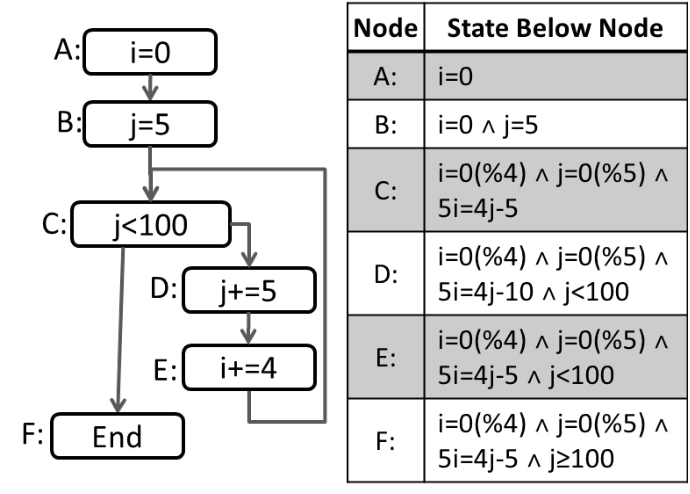
\includegraphics[scale=0.7]{\TutorialExampleDirectory/dfa_ex}
\caption{Example of a dataflow analysis with abstraction of affine constraints.}
\label{Tutorial:dfa_ex}\end{figure}

~\ref{dfa_ex} presents an example with a more complex abstraction: conjunction of linear relationships between variables. At node B the dataflow analysis computes that i=0 and j=5. When this state is propagated through the loop, the analysis discovers that after the first iteration i=4 and j=5. It then computes the meet of i=0 $\wedge$ j=5 and i=4 $\wedge$ j=5, the facts along both paths. Since this abstraction represents linear relationships, the union finds the tightest linear relationships that are true of both input states. It thus infers that i=0 (mod 4), i=0 (mod 5) (i is divisible by 4 and j by 5) and that 5i=4j-5. When this state is propagated again through the body of the loop, these assertions are discovered to be the invariants of this loop and become the fixed-point solution after node C. If they were not invariants, the algorithm would iterate until invariants were found or it reached the abstract state $\top$ which means that no linear constraints are known. Further, since the conditional j\textless100 is also linear, j\textless100 is recorded in the states of the nodes inside the loop and j $\ge$ 100 is recorded at node F after the loop.

\section{ROSE Dataflow Framework}
\label{ROSE_dfa}
ROSE provides a framework for implementing dataflow analyses. It allows users to specify their dataflow analysis by implement the standard dataflow components: (i) an abstraction of the application’s state, (ii) a transfer function that specifies the effects of code on the application state and (iii) a meet operator that combines multiple possible abstract states into one. These are implemented by extending base classes provided by the framework and implementing key virtual methods that correspond to the above functionality. The framework then solves the dataflow equations using the user-provided classes and saves the results at each CFG node. This section describes the functionality provided by the framework and how it can be used to implement analyses. ~\ref{Func_DFA} summarizes the functionality provided by the framework.

\begin{table}
  \centering
  %\tbl{The Functionality of the Dataflow Interface}{
  \scriptsize
  \begin{tabular}{ | p{2cm} | p{2cm} | p{3.5cm} | p{3.5cm} |}
    \hline
    Class & Purpose & Interface & User Responsibilities  \\ \hline
    {\bf Analysis} & Implement Simple CFG passes & Classes {\bf IntraProceduralAnalysis InterProceduralAnalysis} & Extend the classes and implement their {\bf runAnalysis} and {\bf transfer} methods \\ \hline
    {\bf Intra Procedural Dataflow} & Implement intraprocedural dataflow iteration & Classes {\bf IntraFWDataflow} {\bf IntraBWDataflow} & Extend classes and implement {\bf genInitState} and {\bf transfer} methods\\ \hline 
    {\bf Inter Procedural Dataflow} & Implement the inter-procedural dataflow & Classes - {\bf Context Insensitive InterProcedural Dataflow} & Execute on a given instance of {\bf IntraDataflow} \\ \hline
    {\bf Lattice} & Generic interface for abstractions of the application's state & Methods {\bf initialize copy meetUpdate operator== str} & Extend the Lattice class and implement interface methods \\ \hline 
    {\bf Nodestate} & Stores dataflow information of each CFG node & Methods {\bf setLatticeAbove getLatticeAbove deleteLatticeAbove setFact getFact deleteFacts} & Call methods to access dataflow information \\ \hline
    {\bf AstInterface} & Transforms the CFG & Methods {\bf insertBeforeUsing CommaOp, insertAfterUsing CommaOp, replaceWithPattern } & Call methods \\ 
  \hline
  \end{tabular}
%}                                    
  \caption{The Functionality of the Dataflow Interface}
\label{Func_DFA}
\end{table}


\subsection{Call and Control-Flow Graphs}
The ROSE dataflow analysis framework operates on top of the ROSE Call Graph (CG) and Virtual Control-Flow Graph (VCFG). The CG documents the caller/callee relationships between application functions. The VCFG connects SgNodes in the application’s AST to identify the possible execution orders between them. The VCFG is dynamic in that instead of being computing once for the entire application, it computes the outgoing and incoming edges of a given SgNode fresh every time this information is needed. This makes the VCFG very flexible because it automatically responds to changes in the AST with no need for complex adjustments to the graph. 

\subsection{Analyses}
ROSE supports both inter-and intra-procedural analyses. Users implement basic, non-dataflow analyses by extending the {\scriptsize IntraProceduralAnalysis} and {\scriptsize InterProceduralAnalysis} classes. Intra analyses iterate over the CFG of each function, and inter analyses apply intra analyses to individual functions. To implement an analysis an application developer must derive a class from the {\scriptsize IntraProceduralAnalysis} and/or {\scriptsize InterProceduralAnalysis} classes and implement the {\scriptsize runAnalysis} method. Classes {\scriptsize UnstructuredPassInterAnalysis} and {\scriptsize UnstructuredPassIntraAnalysis} {Figure ~\ref{unstruct-ex} provide examples of simple analyses. {\scriptsize UnstructuredPassInterAnalysis} takes as an argument a reference to an {\scriptsize InterProceduralAnalysis} and iterates once through all functions. It applies the {\scriptsize runAnalysis} method of the intra analysis to each function. {\scriptsize UnstructuredPassIntraAnalysis} iterates once through all the CFG nodes in the given function, applying its {\scriptsize visit} method to each node.


\begin{figure}
\centering
\begin{lstlisting}
class UnstructuredPassInterAnalysis : virtual public InterProceduralAnalysis {
  UnstructuredPassInterAnalysis(IntraProceduralAnalysis& intraAnalysis)
  void runAnalysis();
};

class UnstructuredPassIntraAnalysis : virtual public IntraProceduralAnalysis {
   bool runAnalysis(const Function& func, NodeState* state);
   virtual void visit(const Function& func, const DataflowNode& n, 
       NodeState& state)=0;
};  
\end{lstlisting}%
\caption{Example of simple analyses}
\label{unstruct-ex}
\end{figure}

These analyses can be used to implement simple passes through the application’s CFG and serve as the foundation of the dataflow analysis framework. For example, {\scriptsize src/simpleAnalyses/saveDotAnalysis.C} and {\scriptsize src/simpleAnalyses/printAnalysisStates.C} are examples of simple one-pass analyses. {\scriptsize saveDotAnalysis} prints the application’s CFG as a DOT file and {\scriptsize printAnalysisStates} prints the dataflow states of all CFG nodes in the application, which is useful for debugging.

\subsection{Dataflow}
To implement a dataflow analysis in ROSE users must first extend the {\scriptsize Lattice} class to create an abstraction of the application’s state that will be used by the analysis. {\scriptsize Lattices} implement methods such as meet, equality, ordering and operators that allow the {\scriptsize Lattice} to be moved from one lexical scope to another (e.g. from a caller function to the callee). Users then create an intra-procedural analysis by extending the {\scriptsize IntraFWDataflow} to create a forward analysis and from {\scriptsize IntraBWDataflow} to create a backward analysis. Within this class they must implement a function that returns the default abstract state of any given node at the start of the analysis. Further, they implement a {\scriptsize transfer} function that maps the application’s abstract state from before a given CFG node to the state that results from the execution of the node’s expression or statement. Finally, users combine the intra-procedural analysis that they have developed with an inter-procedural analysis of their choice. This analysis will apply the intra-procedural analysis the user has implemented to the application’s functions and resolve the effects of function calls on the application’s abstract state, utilizing the user’s own state abstraction.

For a concrete example, consider how the classical constant-propagation analysis is implemented using ROSE. This analysis uses a simple abstraction of application state, where the abstract state of each variable may be a value the lattice shown in ~\ref{lattice_cpa}

\begin{figure}
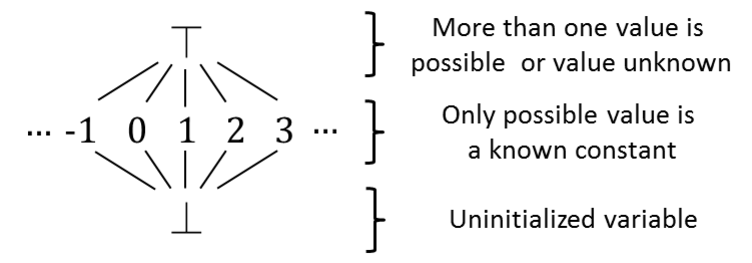
\includegraphics[scale=0.7]{\TutorialExampleDirectory/lattice_cpa}
\caption{Each variable's lattice for constant-propagation analysis}
\label{lattice_cpa}
\end{figure}

The code in below shows a class that implements this lattice. This class derives from the {\scriptsize FiniteLattice} class because the distance between the smallest and largest value in the lattice is finite. Similar functionality is provided for infinite lattices. Its state (lines 4-15) consists of its current level in the lattice as well as its value if the level is {\scriptsize valKnown}. Since the type of {\scriptsize value} is {\scriptsize long}, this abstraction can only represent integral constants. Further, the class has a special {\scriptsize uninitialized} level that means that the object has not yet been used as part of a dataflow analysis. This class implements methods {\scriptsize meetUpdate} (lines 42-65) and the equality operator (lines 68-74) to provide the basic semantics of a lattice. {\scriptsize meetUpdate} computes least upper bound of the constraints in this lattice object and another one, storing the results in this object.If both lattices have the same state, the meet is equal to this state and if they have different states, the meet is $\top$ since the variable represented by the lattice may be set to multiple values on different execution paths. The equality operator determines whether two lattice objects have the same information content. Further, the class implements utility methods that help the dataflow framework manipulate it. The {\scriptsize initialize} method (lines 24-27) ensures the object is ready to be used. Further, two {\scriptsize copy} methods (lines 30-38) make it easy to clone lattice objects. Finally, an {\scriptsize str} method (lines 82-88) simplifies analysis debugging by printing the abstract states at CFG nodes.


%\begin{latexonly}
%   \lstinputlisting{\TutorialExampleDirectory/codesnip_CPA_Lattice.C}
%\end{latexonly}

\begin{frame}
\centering
\begin{lstlisting}
class constPropLat : public FiniteLattice
{
  // The different levels of this object’s lattice
  typedef enum {
    uninitialized=0, // This object is uninitialized
    bottom=1, // No constrains on this object’s value are known
    valKnown=2, // The value of the variable is known (one assignment seen)
    top=3 // This variable may have more than one value
  } latticeLevels;
  
  // The level of this object within its lattice
  latticeLevels level;

  // The value of the variable (if level == valKnown)
  long value;

  nodeConstLattice() { level=uninitialized; }
  
  nodeConstLattice(const nodeConstLattice& that) : 
                              value(that.value), level(that.level) {}

  // Initializes this Lattice to its default state, 
  // if it is not already initialized
  void initialize() {
    if(level == uninitialized)
      level=bottom;
  }
  
  // Returns a copy of this lattice
  Lattice* copy() const { return new nodeConstLattice(*this); }
  
  // Overwrites the state of this Lattice with that of that Lattice
  void copy(Lattice* that) {
    nodeConstLattice* that = dynamic_cast<nodeConstLattice*>(that_arg);
  
    value = that->value;
    level = that->level;
  }

  // Computes the meet of this and that and saves the result in this
  // returns true if this causes this to change and false otherwise
  bool meetUpdate(Lattice* that) {
    // Record this object’s original state to enable change detection
    unsigned long  oldValue = value;
    latticeLevels oldLevel = level;
    
    // Cast that into a nodeConstLattice and abort if this is not possible    
    nodeConstLattice* that = dynamic_cast<nodeConstLattice*>(that_arg);
    ROSE_ASSERT(that);

    // If that is at a higher lattice level than this, the variable must have 
    // multiple possible value on different execution paths
    if(that->level > level) level = top;
    // If both are at the same level
    else if(that->level == level) {
      // If lattices correspond to different values of the variable
      if(level == valKnown && value != that->value)
        level = top; // The union of both these facts is top
    }
    // Otherwise, this lattice doesn’t change
    
    // Return whether this object was modified
    return (oldValID != valID) ||
           (oldLevel != level);
  }
  
  // Equality Operator
  bool operator==(Lattice* that_arg) { 
    // Cast that into a nodeConstLattice and abort if this is not possible    
    nodeConstLattice* that = dynamic_cast<nodeConstLattice*>(that_arg);
    ROSE_ASSERT(that);
    
    return level==that->level && (level!=valKnown || value==that->value);
  }

  // Returns a string representation of this object (this function is 
  // required to simplify debugging)
  string str(string indent="") { … }

  // Sets the state of this lattice to the given value. Returns true if this 
  // causes the lattice's state to change, false otherwise
  bool set(long value)
  {
    bool modified = this->level != valKnown || this->value != value;
    this-> value = value;
    level = valKnown;
    return modified;
  }
}; 
\end{lstlisting}%
\label{unstruct-ex}
\end{frame}


The second step in implementing constant propagation is to provide a class that implements the dataflow analysis itself. This is done by extending the {\scriptsize IntraFWDataflow} class, which implements forward intra-procedural analyses and implementing the {\scriptsize genInitState} and {\scriptsize transfer} methods, described below.

\begin{frame}
\centering
\begin{lstlisting}
class constPropAnalysis : public IntraFWDataflow
{
  constPropAnalysis (): IntraFWDataflow() { }

  // Generates the initial lattice state for the given dataflow node, in the 
  // given function, with the given NodeState
  void genInitState(const Function& func, const DataflowNode& n, 
                    const NodeState& state, vector<Lattice*>& initLattices, 
                    vector<NodeFact*>& initFacts);

  // The transfer function that is applied to every node in the CFG
  // n - The dataflow node that is being processed
  // state - The NodeState object that describes the state of the node, as  
  //         established by earlier analysis passes
  // dfInfo - The Lattices that this transfer function operates on. The 
  //          function takes these lattices as input and overwrites them with 
  //          the result of the transfer.
  // Returns true if any of the input lattices changed as a result of the
  //    transfer function and false otherwise.
  bool transfer(const Function& func, const DataflowNode& n, 
              NodeState& state, const vector<Lattice*>& dfInfo);
}
\end{lstlisting}%
\end{frame}

The {\scriptsize constPropAnalysis} implementation of method {\scriptsize genInitState} creates a lattice (lines 5-7) that maintains the initial abstract state of the application at CFG node {\scriptsize n}. This lattice is an instance of the utility class {\scriptsize FiniteVarsExprsProductLattice}, which creates one copy of {\scriptsize constPropLat} for each variable that is live at node {\scriptsize n}. Since it is a product of lattices, this class is also a lattice with well-defined meet and equality operators based on the operators of its constituent lattices. The dataflow framework provides an identical class for infinite lattices as well as a generic ProductLattice class for arbitrary products of lattices. The function then adds (line 4) the lattice to vector initLattices, which is read by the dataflow framework. This function can also specify one or more facts that the framework will maintain at each node. These facts are not subject to dataflow iteration and can be used to maintain information that is useful independently of the current dataflow state.
 

\begin{frame}
\centering
\begin{lstlisting}
void constPropAnalysis::genInitState(const Function& func, 
              const DataflowNode& n, const NodeState& state,
              vector<Lattice*>& initLattices, vector<NodeFact*>& initFacts) {
  initLattices.push_back(
          new FiniteVarsExprsProductLattice(true, false,  
                                            new constPropLat(), 
                                            NULL, func, n, state));
}
\end{lstlisting}%
\end{frame}

The {\scriptsize transfer} method maps the abstract state before the CFG node n to the state that results from its execution. It begins by accessing the application’s abstract state above node n from the {\scriptsize dfInfo} argument (lines 6-7) . This is the vector of lattices created by {\scriptsize genInitState} for node {\scriptsize n}. It can also be obtained from the {\scriptsize state} object, which maintains the state of the lattices both below and above each node, as well as the facts at each node. The function then initializes all the {\scriptsize constPropLats} in the product lattice (10-13) and advances to analyze the effects of the current node on the abstract state.

Lines 16-127 show how the transfer function operates on different types of {\scriptsize SgNodes}. This code leverages a key feature of how ROSE represents the application’s structure. Since ROSE focuses on source-to-source transformations that minimize the changes in the application’s source code, all analyses must work on the original AST and cannot perform large normalization passes such as transforming the application into SSA form. Since it is difficult to implement complex analyses on top of the AST, we have developed an ``on-demand'' normalization that significantly simplifies the analysis development without changing the AST. Working with AST is difficult because AST sub-trees that describe the structure of expressions are complex and difficult to parse (e.g. consider analyzing all the side-effects of a=b=foo(c=d)). As such, our framework treats every SgExpression that does not correspond to an actual memory object as if it produces a temporary object that is read by its parent {\scriptsize SgExpression}. For example, in the {\scriptsize SgExpression} a=(b=c*5+d), {\scriptsize SgIntVal} 5 produces a temporary variable that is consumed by {\scriptsize SgMultiplyOp c*5. SgVarRefExp c} produces a real application variable, which is also consumed by the {\scriptsize SgMultiplyOp}. The SgMultiplyOp in turn produces a temporary variable that is consumed by {\scriptsize SgAddOp c*5+d}, which produces a temporary variable that is consumed by {\scriptsize SgAssignOp b=c*5+d}, the result of which is consumed by {\scriptsize SgAssignOp a=(b=c*5+d)}. The use of these temporary variables makes it possible for user analyses to focus on just the effects of individual AST nodes without having to analyze sub-trees of the AST. Section~\ref{transfer_analyses} discusses how this on-demand normalization in maintained when updating to the AST. 

The effects of integral constants (e.g. {\scriptsize SgIntVal} or {\scriptsize SgLongLongIntVal}) are transferred on lines 16-31. On line 20 the analysis calls function SgExpr2Var to convert the {\scriptsize SgExpression} into a {\scriptsize varID}, which is an abstract representation of the memory object (either a real or temporary variable) denoted by the {\scriptsize SgExpression}. On line 21 it queries the {\scriptsize FiniteVarsExprsProductLattice} prod with this {\scriptsize varID} to get the {\scriptsize constPropLat} associated with this memory object. If this variable is live (a non-NULL lattice is returned), on lines 26-28 it sets the lattice object to be at level {\scriptsize valKnown} and sets the value to be equal to the constant represented by the {\scriptsize SgExpression}.

 The same logic is used for non-integral constants on lines 33-40. However, since our abstraction cannot represent such constants, their lattices are set to $\top$. Lines 44-60 manage assignments and the lattices of the left-hand-side expression and the assignment {\scriptsize SgAssignOp} itself are set to be equal to the lattice of the right-hand-side expression. The code for variable declaration (lines 63-81) and initialization (lines 84-98) are similar in that the lattice of the right-hand-side is copied to the lattice of the initialized variable. Finally, lines 101-127 focus on arithmetic operations. If the lattices of the left- and right-hand-side expressions are both at levels {\scriptsize valKnown},the operation is performed immediately by the analysis on their statically known values and the result is stored in the lattices of the left-hand-side expression and the {\scriptsize SgExpression} itself. Finally, on line 129 the function returns the {\scriptsize modified} variable, which keeps track of whether the state of the downstream lattices has changed. Since these lattices are inputs to other {\scriptsize SgExpressions}, this informs the dataflow framework whether it needs to analyze how these lattices are transferred by those expressions.   


\begin{frame}
\centering
\begin{lstlisting}
bool constPropAnalysis::transfer(const Function& func, 
                       const DataflowNode& n, 
                       NodeState& state, const vector<Lattice*>& dfInfo) {
  bool modified=false;
  // Get the lattice object
  FiniteVarsExprsProductLattice* prodLat = 
            dynamic_cast<FiniteVarsExprsProductLattice*>(*(dfInfo.begin()));

  // Make sure that all the non-constant Lattices are initialized
  const vector<Lattice*>& lattices = prodLat->getLattices();
  for(vector<Lattice*>::const_iterator it = lattices.begin(); 
      it!=lattices.end(); it++)
    (dynamic_cast<nodeConstLattice*>(*it))->initialize();

  // Integral Numeric Constants
  if(isSgLongLongIntVal(n.getNode())  || 
    // Other types of integral constants 
    ...) {
    // Memory object and lattice of the expression’s result
    varID res = SgExpr2Var(isSgExpression(n.getNode()));
    constPropLat* resLat = dynamic_cast<constPropLat*>(
                                                prodLat->getVarLattice(res));

    // If the result expression is live
    if(resLat) {
      if(isSgLongLongIntVal(n.getNode()))
        modified = resLat->set(isSgLongLongIntVal(n.getNode())->get_value()) 
                   || modified;
      // Same for other types of integral constants 
      ...
    }
  // Non-integral Constants
  } else if(isSgValueExp(n.getNode())) {
    // Memory object and lattice of the expression’s result
    varID res = SgExpr2Var(isSgExpression(n.getNode()));
    constPropLat* resLat = dynamic_cast<constPropLat*>(
                                                prodLat->getVarLattice(res));
    // If the result expression is live, set it to top since we only work 
    // with integral constants
    if(resLat) modified = resLat->setTop() || modified;

  // Plain assignment: lhs = rhs
  } else if(isSgAssignOp(n.getNode())) {
    // Memory objects denoted by the expression’s left- and right-hand   
    // sides as well as the SgAssignOp itself
    varID lhs = SgExpr2Var(isSgAssignOp(n.getNode())->get_lhs_operand());
    varID rhs = SgExpr2Var(isSgAssignOp(n.getNode())->get_rhs_operand());
    varID res = SgExpr2Var(isSgExpression(n.getNode()));

    // The lattices associated the three memory objects
    constPropLat* resLat = 
            dynamic_cast<constPropLat*>(prodLat->getVarLattice(res));
    constPropLat* lhsLat = 
            dynamic_cast<constPropLat*>(prodLat->getVarLattice(lhs));
    constPropLat* rhsLat = 
            dynamic_cast<constPropLat*>(prodLat->getVarLattice(rhs));

    // If the lhs and/or the SgAssignOp are live, copy lattice from the rhs
    if(lhsLat){ lhsLat->copy(rhsLat); modified = true; }    
    if(resLat){ resLat->copy(rhsLat); modified = true; }    

  // Variable Declaration
  } else if(isSgInitializedName(n.getNode())) {
    varID var(isSgInitializedName(n.getNode()));
    constPropLat* varLat = dynamic_cast<constPropLat*>(
                                               prodLat->getVarLattice(var));

    // If this variable is live
    if(varLat) {
      // If there was no initializer, initialize its lattice to Bottom
      if(initName->get_initializer()==NULL)
        modified = varLat->setBot() || modified;
      // Otherwise, copy the lattice of the initializer to the variable
      else {
        varID init = SgExpr2Var(
                        isSgInitializedName(n.getNode())->get_initializer());
        ConstPropLat* initLat = dynamic_cast<ConstPropLat*>(
                                               prodLat->getVarLattice(init));
        if(initLat) { varLat->copy(initLat); modified = true; }
      }
    }

  // Initializer for a variable
  } else if(isSgAssignInitializer(n.getNode())) {
    // Memory objects of the initialized variable and the 
    // initialization expression
    varID res = SgExpr2Var(isSgAssignInitializer(n.getNode()));
    varID asgn = SgExpr2Var(isSgAssignInitializer(
                                         n.getNode())->get_operand());

    // The lattices associated both memory objects
    constPropLat* resLat = 
            dynamic_cast<constPropLat*>(prodLat->getVarLattice(res));
    constPropLat* asgnLat = 
            dynamic_cast<constPropLat*>(prodLat->getVarLattice(asgn));

    // If the variable is live, copy lattice from the assignment
    if(resLat){ resLat->copy(asgnLat); modified = true; }

  // += Arithmetic Operation
  } else if(isSgPlusAssignOp(n.getNode())) {
    // Memory objects denoted by the expression’s left- and right-hand   
    // sides as well as the SgAssignOp itself
    varID lhs = SgExpr2Var(isSgAssignOp(n.getNode())->get_lhs_operand());
    varID rhs = SgExpr2Var(isSgAssignOp(n.getNode())->get_rhs_operand());
    varID res = SgExpr2Var(isSgExpression(n.getNode()));

    // The lattices associated the three memory objects
    constPropLat* resLat = 
            dynamic_cast<constPropLat*>(prodLat->getVarLattice(res));
    constPropLat* lhsLat = 
            dynamic_cast<constPropLat*>(prodLat->getVarLattice(lhs));
    constPropLat* rhsLat = 
            dynamic_cast<constPropLat*>(prodLat->getVarLattice(rhs));

    // If the lhs and/or the SgAssignOp are live and we know both their 
    // values of the value of the rhs expression, set their lattice to be the     
    // sum of the two.
    if(lhsLat && lhsLat->level==constPropLat::valKnown && 
       rhsLat->level==constPropLat::valKnown)
    { modified = lhsLat->set(lhsLat->value + rhsLat->value) || modified; }
    if(resLat && resLat->level==constPropLat::valKnown && 
       rhsLat->level==constPropLat::valKnown)
    { modified = resLat->set(resLat->value + rhsLat->value) || modified; }
  } 
  // Same for other arithmetic operations
  ...

  return modified;
}
\end{lstlisting}%
\end{frame}
Once the intra-procedural analysis has been implemented, it can be executed on the application by combining it with an inter-procedural analysis. Currently two such analyses are implemented. {\scriptsize ContextInsensitiveInterProceduralDataflow} implements a basic context-insensitive analysis that propagates abstract state from callers to callees but does not differentiate between different call sites of the same function. As such, it is sensitive to inter-procedural data flows but can be imprecise because it takes into account control flows that are actually impossible, such as entering a function from one call site but returning to another. The code below provides an example of how this analysis is used to create an inter-procedural constant propagation analysis. The dataflow framework is initialized on line 6 and the application’s call graph is built on lines 9-11. The intra-procedural analysis object is created on line 17 and the context-insensitive inter-procedural analysis is created on line 20. The user passes into its constructor references to their intra-procedural analysis and the call graph. Finally, on line 23 the user applies the full inter-procedural analysis to the entire application. 
 
\begin{frame}
\centering
\begin{lstlisting}
int main( int argc, char * argv[] )  {
  // Build the AST used by ROSE
  SgProject* project = frontend(argc,argv);
  
  // Initialize the ROSE dataflow framework
  initAnalysis(project);

  // Build the call graph
  CallGraphBuilder cgb(project);
  cgb.buildCallGraph();
  SgIncidenceDirectedGraph* graph = cgb.getGraph(); 

  // Set the debug level to print the progress of the dataflow analysis
  analysisDebugLevel = 1;
  
  // Create the intra-procedural constant propagation analysis
  constPropAnalysis cp(project);

  // Create the inter-procedural analysis for intra-analysis cp
  ContextInsensitiveInterProceduralDataflow inter_cp(&cp, graph);

  // Run inter-procedural constant propagation on the entire application
  inter_cp.runAnalysis();
}
\end{lstlisting}
\end{frame}

To simplify debugging the framework also provides the {\scriptsize UnstructuredPassInterDataflow} analysis, which simply applies the user’s intra-procedural analysis on each function within the application. While this produces globally incorrect results, it simplifies debugging analyses on individual functions. 

\subsection{Transferring Information Between Analyses}
\label{transfer_analyses}
Since in practice users need to implement multiple analyses where one depends on the results of another, the ROSE dataflow framework maintains the results of all analyses at each CFG nodes and makes it easy for analyses to access this data. The lattices and facts of a given CFG node are stored in its associated {\scriptsize NodeState} object. The data produced by an analysis can be retrieved by using its pointer, as shown in the example below.

This code shows analysis {\scriptsize exAnalysis}, which takes in its constructor a pointer to the {\scriptsize constPropAnalysis} described above (lines 4-5). Inside its transfer function this analysis calls the {\scriptsize getLatticeBelow} method of its argument state (instance of the {\scriptsize NodeState} class) to get the lattice associated with {\scriptsize constPropAnalysis} that has index 0 (lines 11-13). It then gets the {\scriptsize constPropLat} of any variable it cares about and make analysis decisions based on what is statically known about its state.

\begin{frame}
\centering
\begin{lstlisting}
class exAnalysis {
  // Class maintains a pointer to the constant propagation analysis to make 
  // it possible to access its results
  constPropAnalysis& cpAnalysis;
  exAnalysis(constPropAnalysis* cpAnalysis) : cpAnalysis (cpAnalysis) {}

  bool transfer(const Function& func, const DataflowNode& n, 
                NodeState& state, const vector<Lattice*>& dfInfo) {
    // Get the Lattices computed by the constant propagation analysis for the 
    // current CFG node
    FiniteVarsExprsProductLattice* prodLat = 
               dynamic_cast<FiniteVarsExprsProductLattice*>(
                                      state->getLatticeBelow(cpAnalysis, 0));

    // Some application variable of interest
    varID var = ...;

    // The constPropLat of this variable
    constPropLat varCPLat = dynamic_cast<constPropLat*>(
                                                prodLat->getVarLattice(res));

    // Analyze differently depending on what is known about the 
    // variable’s value 
    if(varCPLat) 
      if(varCPLat->level == constPropLat::bottom) {
        ...
      } else if(varCPLat->level == constPropLat::valKnown) {
        ...
      } else if(varCPLat->level == constPropLat::top) {
        ...
      }
  }
  ...
};
\end{lstlisting}
\end{frame}

The code below shows the full functionality of the {\scriptsize NodeState} class. . Lines 5-16 show the functions to set, get and delete the lattices above and below the associated CFG node.  Lines 20-26 provide the same functionality for facts. The {\scriptsize str} method on line 20 returns a string representation of the lattices and facts associated with the CFG node, which is very useful for debugging. Lines 37-50 show the object’s static methods. The {\scriptsize getNodeState} method on line 37 returns the {\scriptsize NodeState} object of a given CFG node. Since the ROSE virtual CFG can have multiple CFG nodes for the same AST node, this method requires an additional index argument to identify the node in question. Finally, method copyLattices\_aEQa and related methods (lines 39-50) copy lattice information from above a CFG node to below it and vice versa, from one node to another or from one analysis at a given node to another analysis at the same node.  

\begin{frame}
\centering
\begin{lstlisting}
class NodeState
{
  // Sets the lattices above/below this node for the given analysis to the   
  // given lattice vector
  void setLatticeAbove(const Analysis* analysis, vector<Lattice*>& lattices);
  void setLatticeBelow(const Analysis* analysis, vector<Lattice*>& lattices);
  
  // Returns the lattice latticeName generated by the given analysis from 
  // above/below the node
  Lattice* getLatticeAbove(const Analysis* analysis, int latticeName) const;
  Lattice* getLatticeBelow(const Analysis* analysis, int latticeName) const;
  
  // Deletes all lattices above/below this node that are associated with the 
  // given analysis
  void deleteLatticeAbove(const Analysis* analysis);
  void deleteLatticeBelow(const Analysis* analysis);
  
  // Sets the facts at this node for the given analysis to the given 
  // fact vector
  void setFacts(const Analysis* analysis, const vector<NodeFact*>& newFacts);
  
  // Returns the given fact, owned by the given analysis
  NodeFact* getFact(const Analysis* analysis, int factName) const ;
  
  // Deletes all facts at this node associated with the given analysis
  void deleteFacts(const Analysis* analysis);

  // Returns a string representation of all the lattices and facts 
  // associated with the CFG node
  string str(Analysis* analysis, string indent) const;

  // --- Static Methods --- 
  // Returns the NodeState object associated with the given dataflow node
  // index is used when multiple NodeState objects are associated with a 
  // given node
  // (ex: SgFunctionCallExp has 3 NodeStates: entry, function body, exit)
  static NodeState* getNodeState(const DataflowNode& n, int index=0);
    
  // Copies from's above lattices for the given analysis to to's above 
  // lattices for the same analysis
  static void copyLattices_aEQa(Analysis* analysis, NodeState& to, const 
                                NodeState& from);
  
  // Copies from's above lattices for analysisA to to's above lattices for 
  // analysisB
  static void copyLattices_aEQa(Analysis* analysisA, NodeState& to, 
                                Analysis* analysisB, const NodeState& from);
  
  // Similar methods for copying in different permutations
  ...
};
\end{lstlisting}
\end{frame}

\subsection{CFG Transformations}
ROSE makes it easy to modify the application’s AST as a result of dataflow analyses. The dataflow framework maintains an on-demand normal form, where analyses can focus on the actions of individual SgNodes and ignore how they are arranged within the AST. ROSE maintains this abstraction by providing an API that inserts new SgExpressions into the application’s CFG, making all the needed changes in the AST to make sure that the correct control flow is maintained. 


\begin{figure}
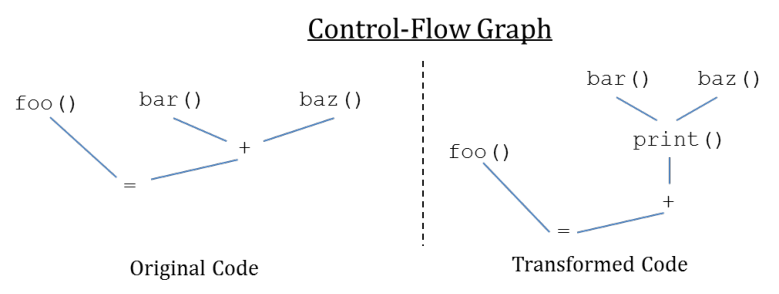
\includegraphics[scale=0.7]{\TutorialExampleDirectory/transformation_cfg.pdf}
\caption{Example of Transformation on the CFG}
\label{tr_cfg}
\end{figure}

To get the intuition of this functionality consider the expression {\scriptsize foo()=(bar()+baz())}. Suppose the user has decided based on the dataflow state before the {\scriptsize SgAddOp +} that it they want to add a call to function {\scriptsize print} immediately before it. From the perspective of the CFG, this is a simple and well-defined operation, as shown at the top of Figure 4. The side-effects of the calls to {\scriptsize bar} and {\scriptsize baz} must complete before the call to print and the side-effects of print must complete before the execution of the + operation. The call to {\scriptsize foo} is not well-ordered relative print or the other operations by the structure of the CFG.

Unfortunately, it is difficult to implement these semantics in the context of the AST because (i) there is no way to add a function call to an {\scriptsize SgAddOp} and (ii) because in C++ the sequence points required by the above semantics (some side-effects much complete before others) are provided by a few specific constructs such as statement boundaries and the comma operator. As such, the transformation requires the complex set of AST changes shown in the Figure 5. We must create temporary variables to hold the results of the calls to bar and baz. We then transform the original {\scriptsize SgAddOp} into a longer {\scriptsize SgCommaOpExp}, where we first call {\scriptsize bar} and {\scriptsize baz}, saving their results into the temporary variables, then call print and finally perform the addition. The result of the addition is the result of the entire comma expression, so this transformation correctly enforces the semantics of the desired transformation.


\begin{figure}
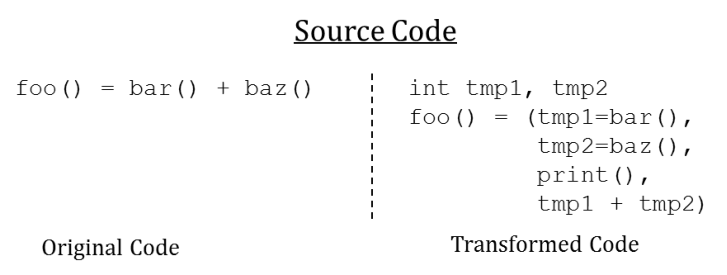
\includegraphics[scale=0.7]{\TutorialExampleDirectory/transformation_srcode.pdf}
\caption{Example of the Transformation on the Source Code}
\label{tr_srcode}
\end{figure}

ROSE provides the three functions to make it easy to insert expressions into the CFG. Functions {\scriptsize insertBeforeUsingCommaOp} and {\scriptsize insertAfterUsingCommaOp} insert {\scriptsize SgExpressions} before or after existing {\scriptsize SgExpressions} using a generalization of the transformation described in Figure ~\ref{tr_srcode}. 

\begin{frame}
\centering
\begin{lstlisting}
// Insert an expression (new_exp) before another expression (anchor_exp) has 
// possible side effects, without changing the original semantics. This is 
// achieved by using a comma operator: (new_exp, anchor_exp). The comma 
// operator is returned.
SgCommaOpExp *insertBeforeUsingCommaOp(SgExpression* new_exp, 
                                       SgExpression* anchor_exp);
// Insert an expression (new_exp) after another expression (anchor_exp) has 
// possible side effects, without changing the original semantics. This is 
// done by using two comma operators:  
//     type T1; ... ((T1 = anchor_exp, new_exp),T1) )... , 
// where T1 is a temp variable saving the possible side effect of anchor_exp. 
// The top level comma op exp is returned. The reference to T1 in T1 = 
// anchor_exp is saved in temp_ref.
SgCommaOpExp *insertAfterUsingCommaOp(SgExpression* new_exp, 
                    SgExpression* anchor_exp, SgStatement** temp_decl = NULL, 
                    SgVarRefExp** temp_ref = NULL);
\end{lstlisting}%
\label{insert-ex}
\end{frame}

Function replaceWithPattern (Figure~\ref{rep}) replaces one SgExpression with another. However, since the original expression may still be valuable, it allows the original expression to be included at one or more locations inside the new expression that contain nodes of type SgVariantExpression. 


\begin{frame}
\centering
\begin{lstlisting}
// Replace an anchor node with a specified pattern subtree with optional 
// SgVariantExpression. All SgVariantExpression in the pattern will be 
// replaced with copies of the anchor node.
SgNode* replaceWithPattern (SgNode * anchor, SgNode* new_pattern);
\end{lstlisting}%
\label{rep}
\end{frame}

An example of this transformation is shown Figure~\ref{cfg-srcode}, where the original code is the same as in the example above and the {\scriptsize new\_pattern} expression is a single {\scriptsize SgMultOp} where the arguments are both {\scriptsize SgVariantExpressions}. The result of the transformation is that the original {\scriptsize SgAddOp} is replaced with a multiplication the arguments of which are copies of the {\scriptsize SgAddOp: (bar()+baz())*(bar()+baz())}.


\begin{figure}
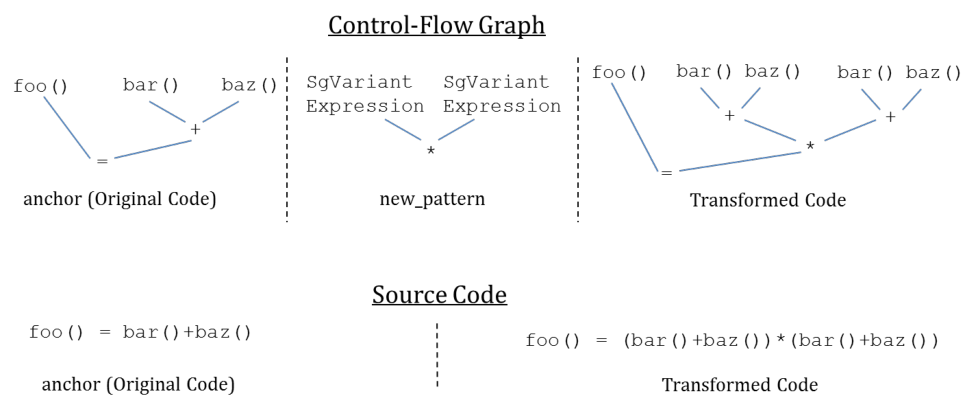
\includegraphics[scale=0.7]{\TutorialExampleDirectory/code_replacement_transformation.pdf}
\caption{Code Replacement Transformation}
\label{cfg-srcode}
\end{figure}

